%*******************************************************************************
%****************************** Second Chapter *********************************
%*******************************************************************************

\chapter{Introduction}

\graphicspath{{Figs/}}

%********************************** %First Section  **************************************

\section{Introduction to LHCb and VELO} %Section - 1.1 

\begin{figure}[h] % h for here in document
\centering
\begin{subfigure}[t]{0.45\textwidth}
\centering
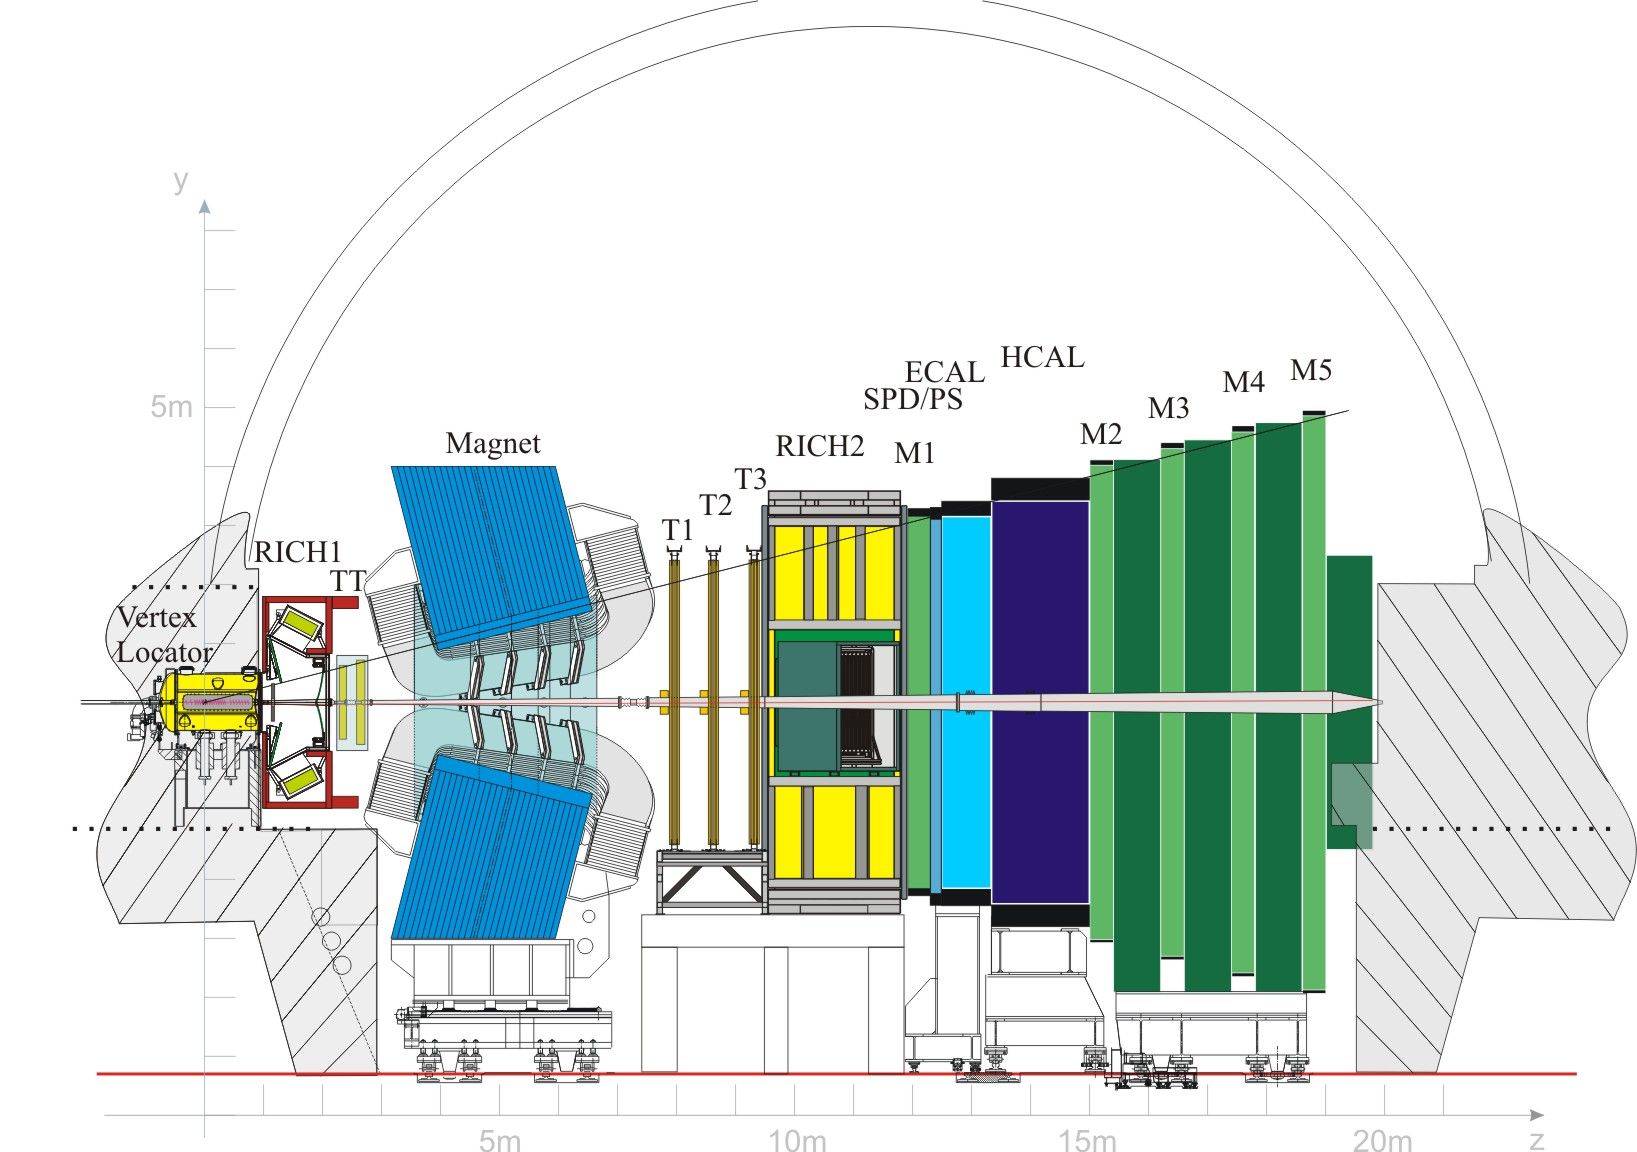
\includegraphics[width=\textwidth]{LHCbDiagram}
\caption{Diagram of LHCb detector, the VELO is on the far left. More tracking modules and calorimeters make up the detector.} 
\label{fig:LHCbDiagram} 
\end{subfigure}
~
\begin{subfigure}[t]{0.45\textwidth}
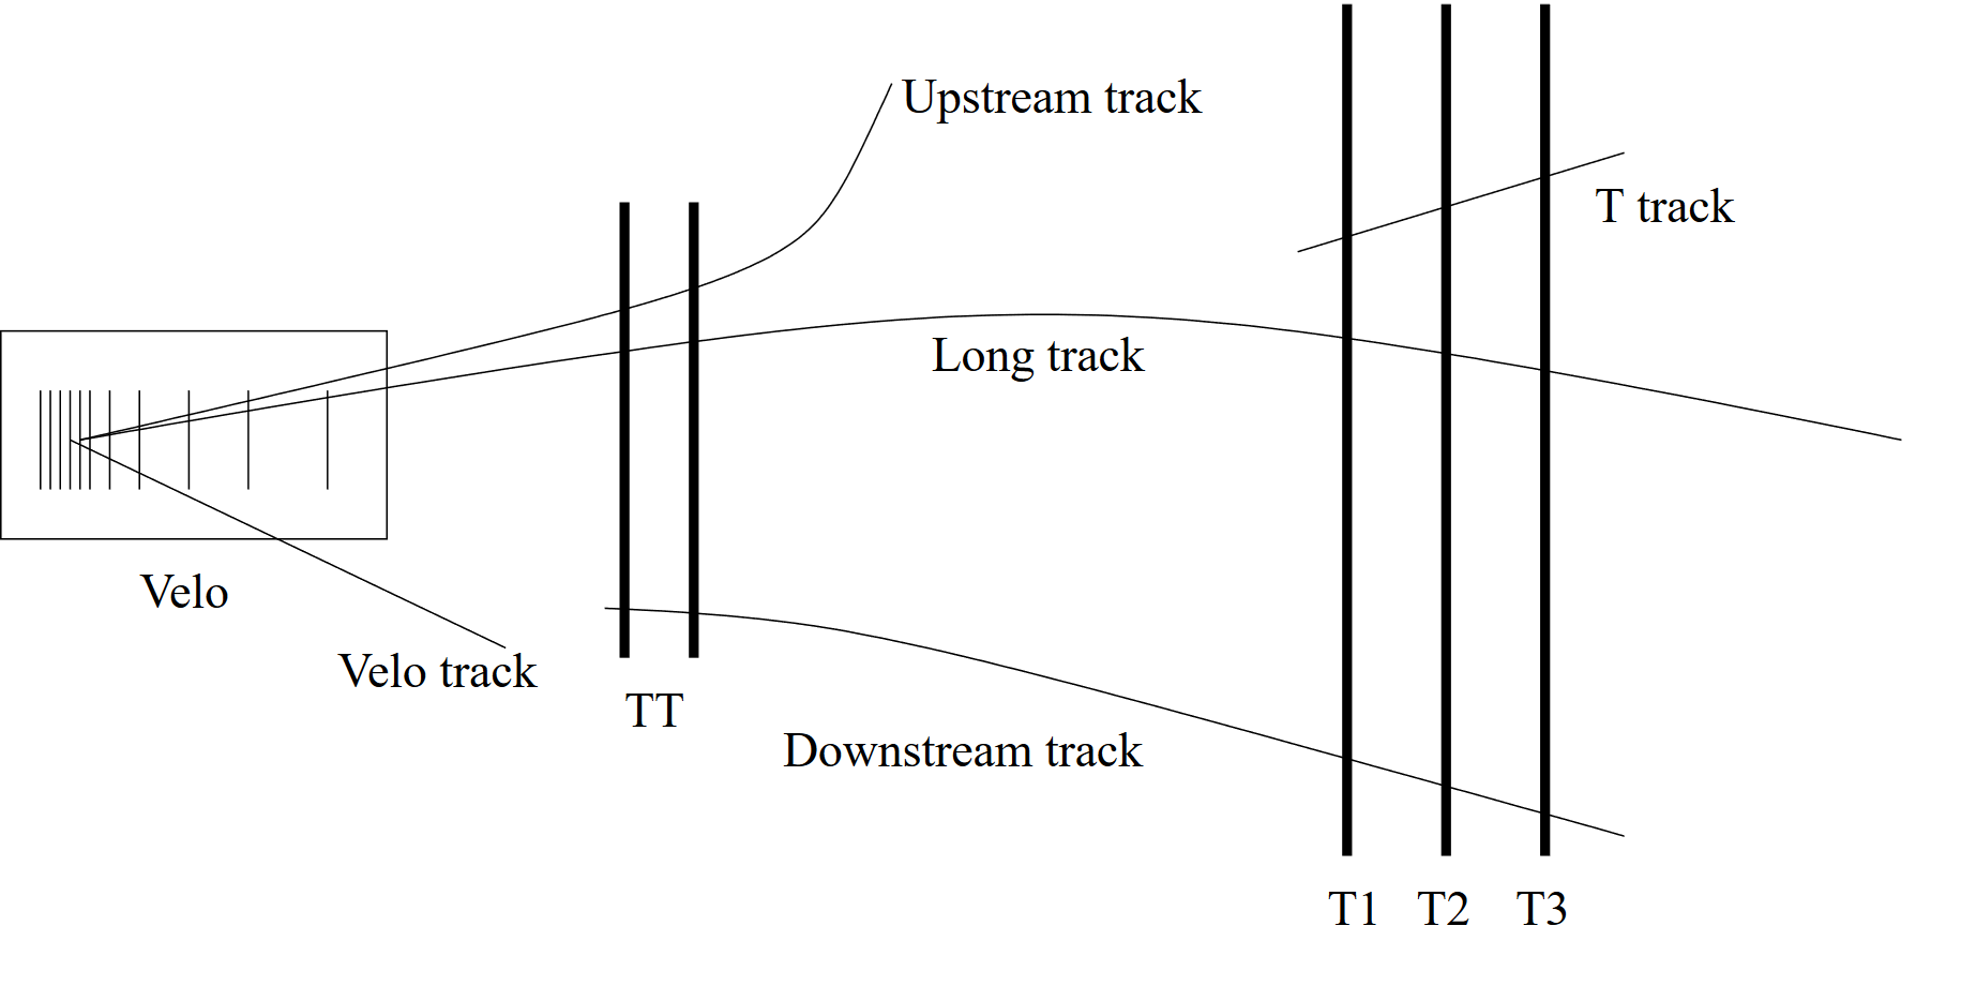
\includegraphics[width=\textwidth]{LHCbTracking}
\caption{Types of tracks found by LHCb} 
\label{fig:LHCbTracking}
\end{subfigure}
\end{figure}

\begin{figure}[h] % h for here in document
\centering
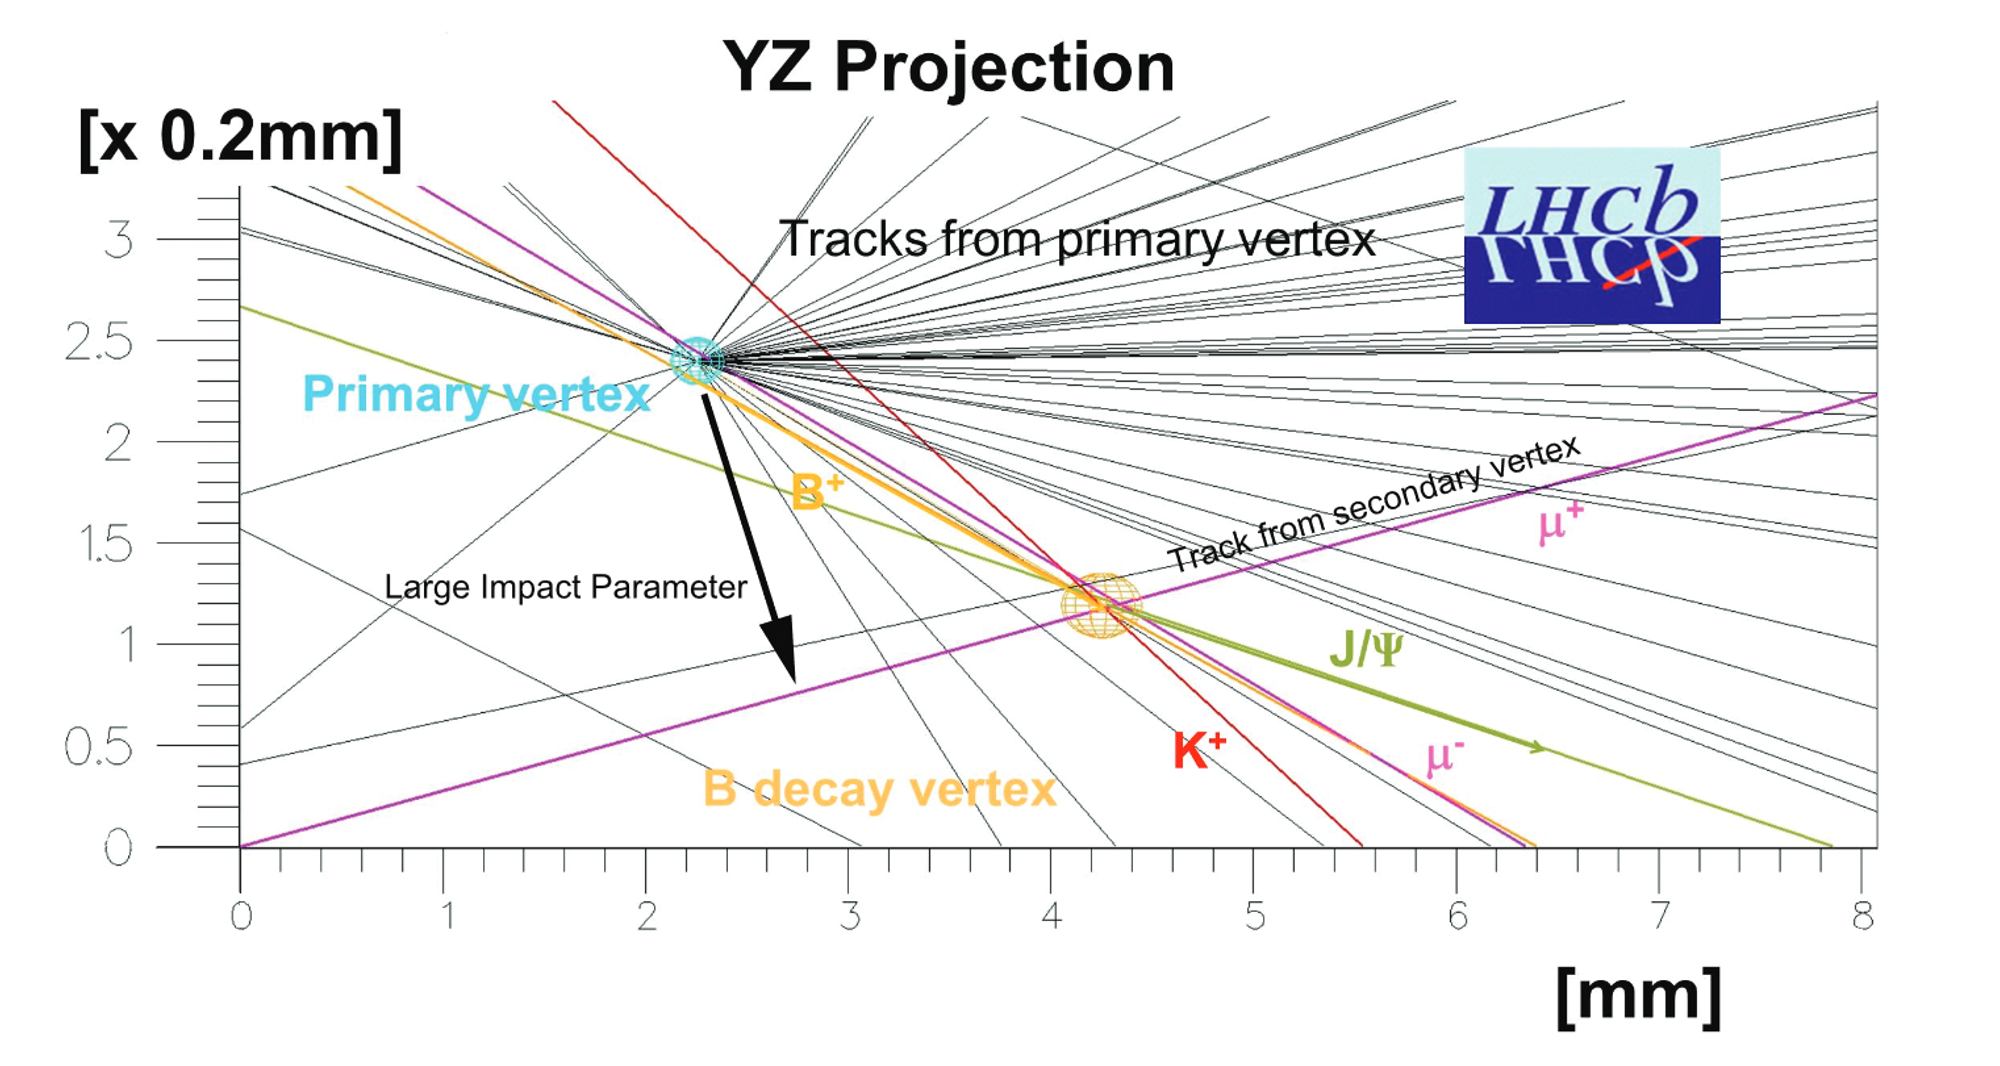
\includegraphics[width=\textwidth]{EventDiagram.png}
\caption{Diagram of typical LHCb event.} 
\label{fig:EventDiagram} 
\end{figure}

LHCb is a single-arm forward spectrometer at the Large Hadron Collider. It is designed to study heavy flavour physics and covers a pseudorapidity range of $2 < \eta < 5$. It has pioneered the search for CP violation, as well as Electroweak physics in forward direction. The experiment was designed for indirect searches of new particles, enhancing rare decay branching fractions and for precise measurements of standard model parameters \citep{Collaboration2008TheLHC}. The design of LHCb is shown in figure \ref{fig:LHCbDiagram}. Unlike other LHC experiments LHCb does not look in all directions around the collision point, instead it looks in the forward region only, with the collision point at one end of the experiment. At this collision point is positioned the Vertex Locator (VELO). Vertex location is fundamental to the success of LHCb \citep{Barbosa-Marinho:504321}. A vertex is the point in space that particles are created or decay. b-meson decays, which LHCb searches for, have distinctive displaced secondary vertices which must be correctly identified to determine decay lifetimes and tag flavours of particles. The primary vertex is the point of the first collision, at the LHC this is the proton-proton (pp) collision. A secondary vertex is the point of decay of products of the first decay. b-meson decays are identified by their impact parameter (IP), the distance between the primary vertex and the nearest point on the track \cite{Kucharczyk:1756296} see figure \ref{fig:LHCbTracking}. Primary vertices are found from tracks reconstructed by the VELO. A track is a series of connected hits in the detector that were created by the same particle, correctly reconstructing tracks from hits in the detector can be used to identify particle momenta as well as finding Primary Vertices. Types of tracks found by LHCb are shown in figure \ref{fig:EventDiagram} \cite{LHCb2012TrackingLHCb}. Reconstructing tracks in the VELO is the primary aim of this project. Pattern recognition is the method used to identify which hits were caused by each particle, and correctly group them into tracks.

%********************************** % Second Section  *************************************

\section{The LHCb and VELO Upgrade}  %Section - 1.2

The current VELO has been in operation since the start of LHC operation in 2008, however as part of the LHCb upgrade a new VELO is being constructed. The LHCb upgrade is scheduled for run-III in 2021 \cite{Hennessy2016LHCbUpgrade} and involves upgrades to many parts of the experiment. 
% Write something about what LHCb wants to measure in the future
The headline feature of the LHCb upgrade is the 5 times increase of luminosity to \(2\times10^{33} cm^{-2} s^{-1}\), this increase will require to the removal of the L0 hardware trigger, this will increase event rate from the current 1MHz to the full 40MHz event rate capable at the LHC \cite{Collaboration:1624070}. The current software triggers will also be replaced. These changes will result in more events occurring in the experiment, and more information about these events being read. For the VELO this will mean higher pile-up per event and more events per second, it can be seen therefore that the speed of pattern recognition algorithms must be greatly increased to cope.
The current VELO is a silicon strip detector consisting of 42 modules positioned around the LHCb interaction point over a range of approximately 1m shown in figure \ref{fig:CurrentVelo}. Each module contains silicon strip sensors and is split in half so that the detector can be retracted during beam injection. This is required because the VELO sensors are designed to be positioned millimetres from the beam line, during beam injection the beam is not perfectly centred, and could cause damage to the sensors. 
The upgraded VELO has a similar basic design but with many important differences figure \ref{fig:UpgradeVELO}. The number of modules will be increased to 52, and importantly the silicon strip sensors are being changed to pixel sensors. These sensors will be placed closer to the beam, just 5.1mm away compared to 8.2mm of the current VELO. Finally the new electronics will readout the sensors at 40MHz, giving a total VELO data rate of 1.2Tb/s, greatly increased from the 150Gb/s of the current VELO \cite{Hennessy2016LHCbUpgrade}. 
A diagram of a pair of modules is shown in figure \ref{fig:VeloSensorDiagram}. The VELO pixel sensors are 2d arrays of 256x256 pixels, three sensors are placed side by side to create effective 768x256 arrays. 2 of these arrays are positioned in an L shape on each side of each module. When the pair of modules are in the closed position they form an almost square array of pixel sensors \cite{Bird:1620453}. In reality these are rotated by 45 degrees.

\section{Motivation}
The LHCb upgrade will see a vast increase in data rate. If current computing systems are kept in place for Run III then storage capacity and computing power requirements will exceed current capacity by an order of magnitude\cite{Bozzi:2298181}. However it will not be as simple as increasing computing capacity to cope as this is not likely to be funded. Therefore work must be done to ensure upgrade software is more efficient. Trigger performance was improved for Run II by means of a second High Level Trigger (HLT2), allowing physics analysis to be done directly from objects directly out of the trigger. Event data size has also been reduced using the \verb|Turbo| stream, which stores only some information about events.\\
For Run III further performance gains can be achieved by maximising the use of parallel computing on multi-core systems and GPU's. This will involve major changes to software to utilise these benefits.


\begin{figure}[ht] % h for here in document
\centering
\begin{subfigure}[t]{0.45\textwidth}
\centering
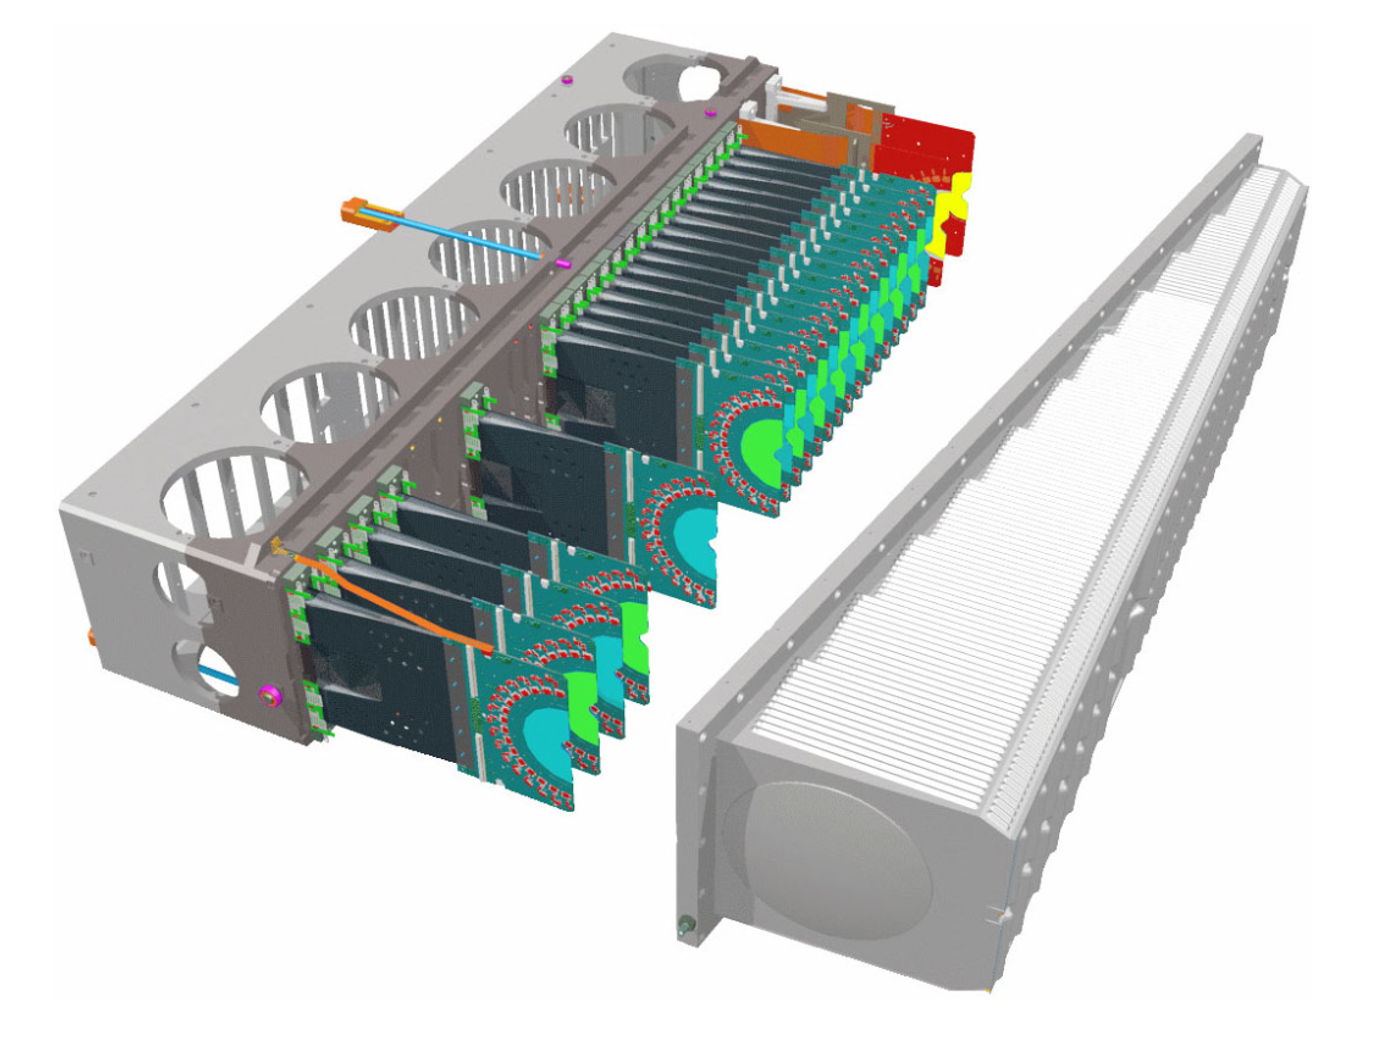
\includegraphics[width=\textwidth]{CurrentVelo}
\caption{Diagram of current VELO.} 
\label{fig:CurrentVelo} 
\end{subfigure}
~
\begin{subfigure}[t]{0.45\textwidth}
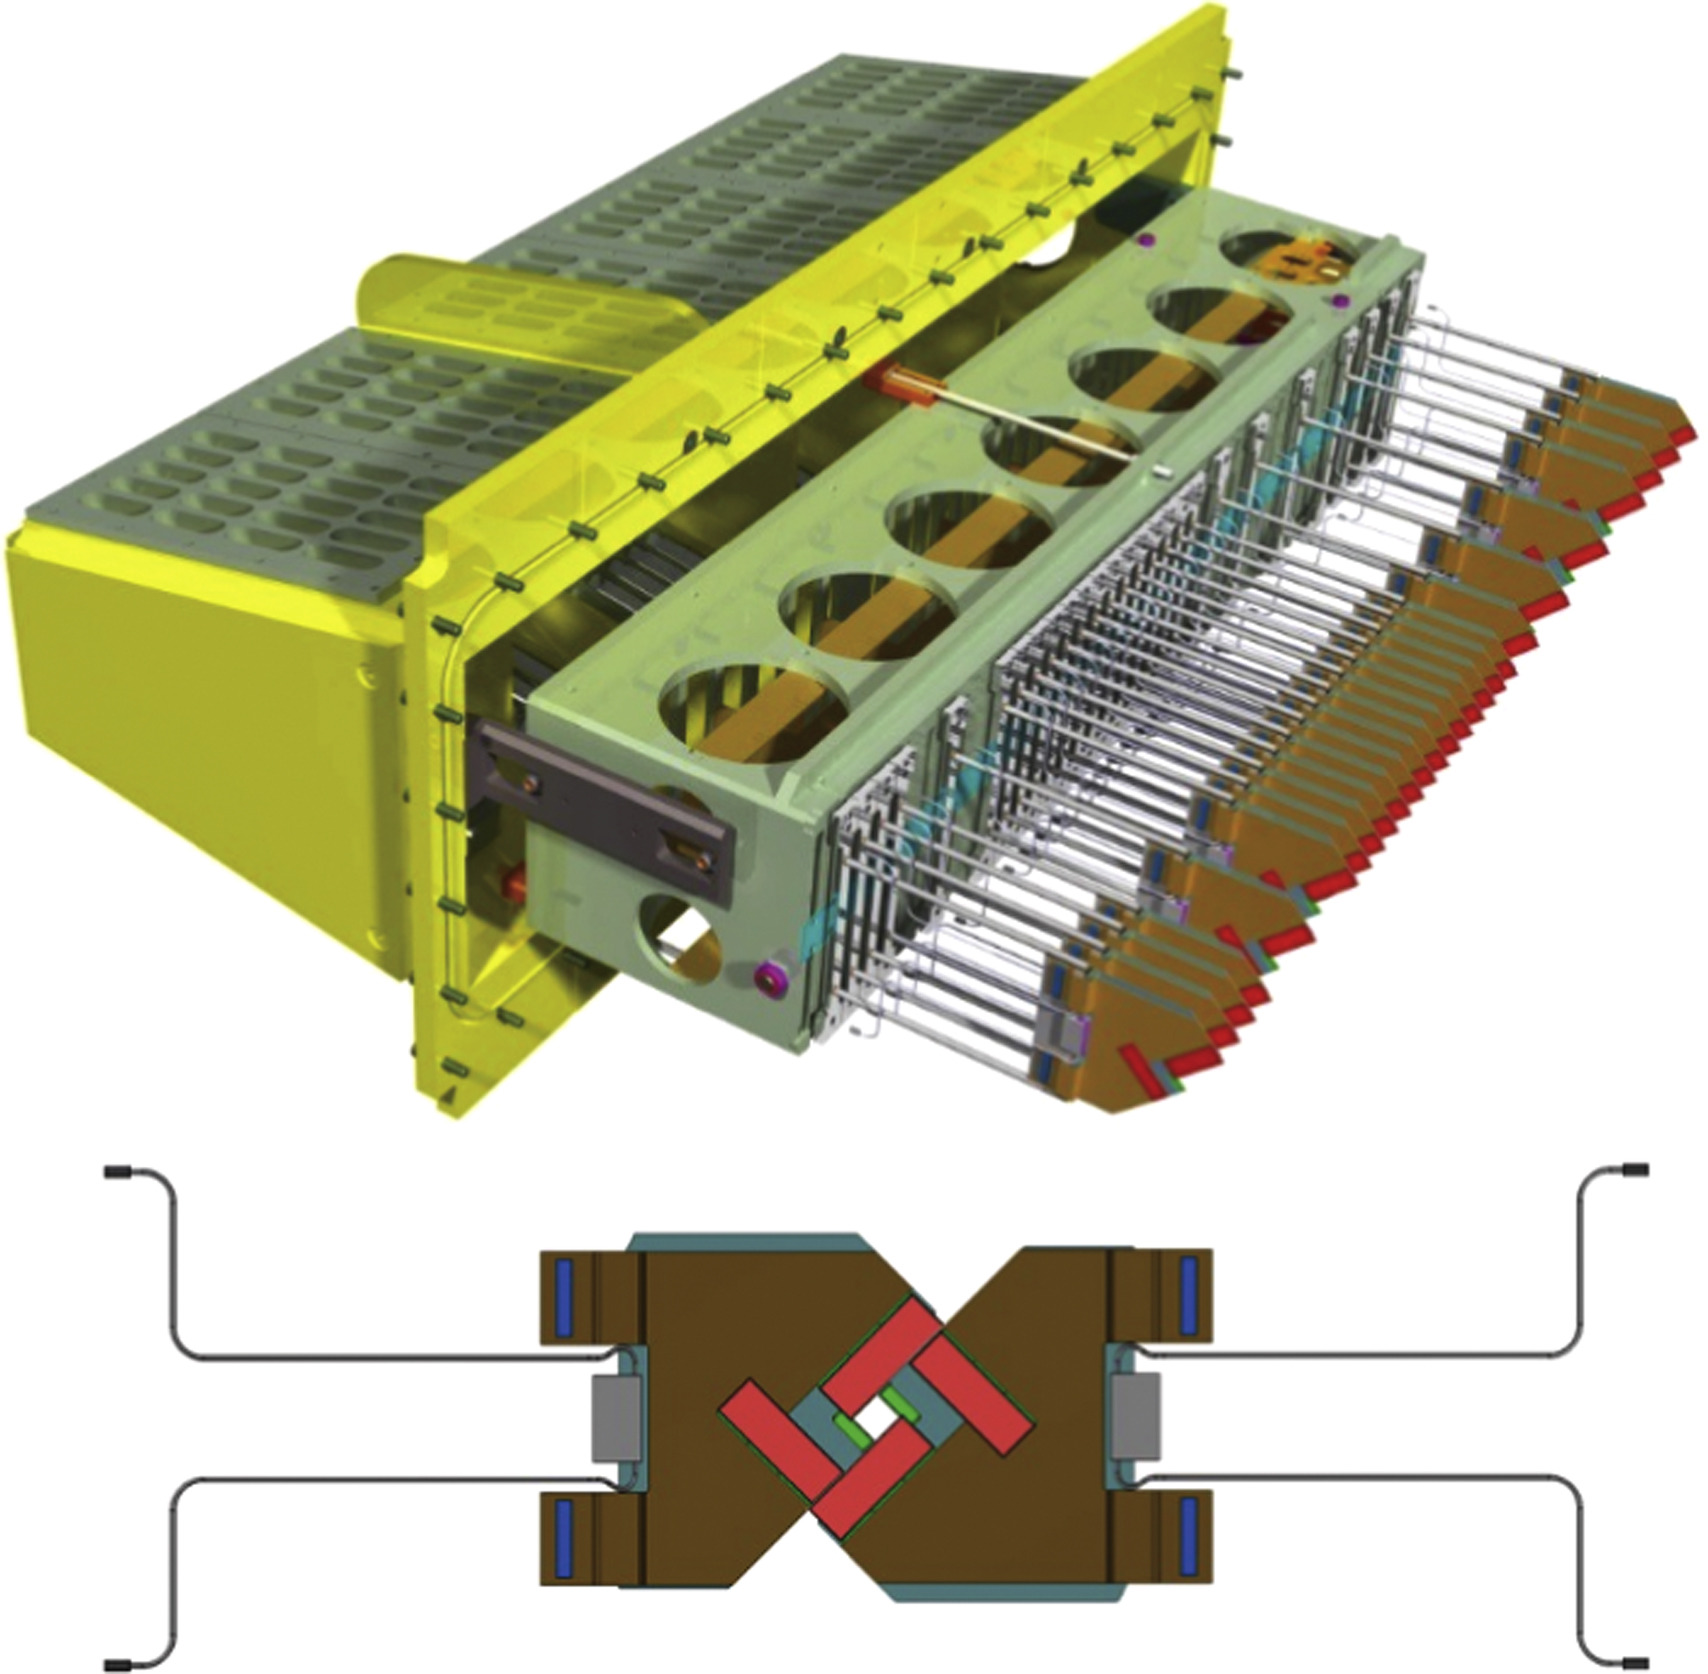
\includegraphics[width=\textwidth]{UpgradeVELO}
\caption{Diagram of upgrade VELO.} 
\label{fig:UpgradeVELO}
\end{subfigure}
\end{figure}

\begin{figure}[ht] % h for here in document
\centering
\begin{subfigure}[t]{0.45\textwidth}
\centering
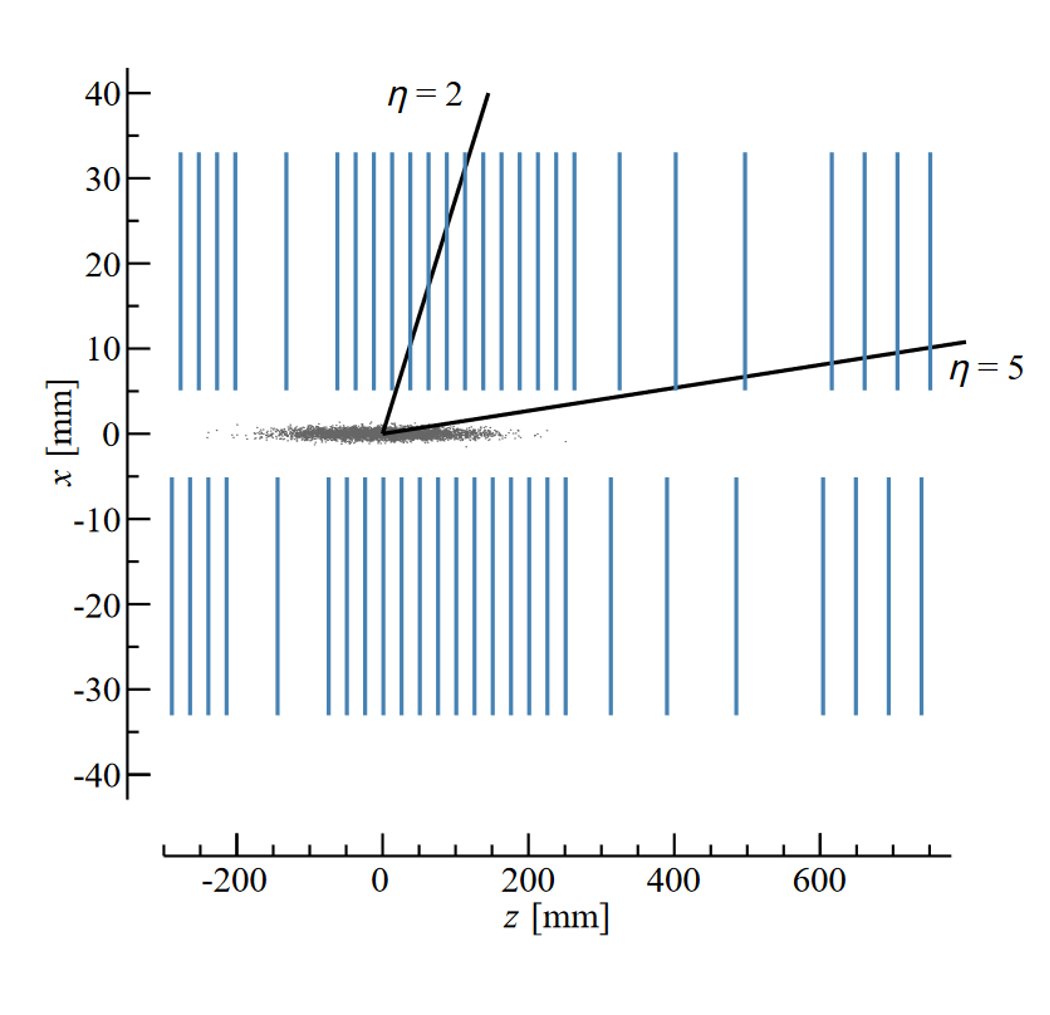
\includegraphics[width=\textwidth]{VeloLayerDiagram}
\caption{Diagram of VELO upgrade module layout.} 
\label{fig:VeloLayerDiagram} 
\end{subfigure}
~
\begin{subfigure}[t]{0.45\textwidth}
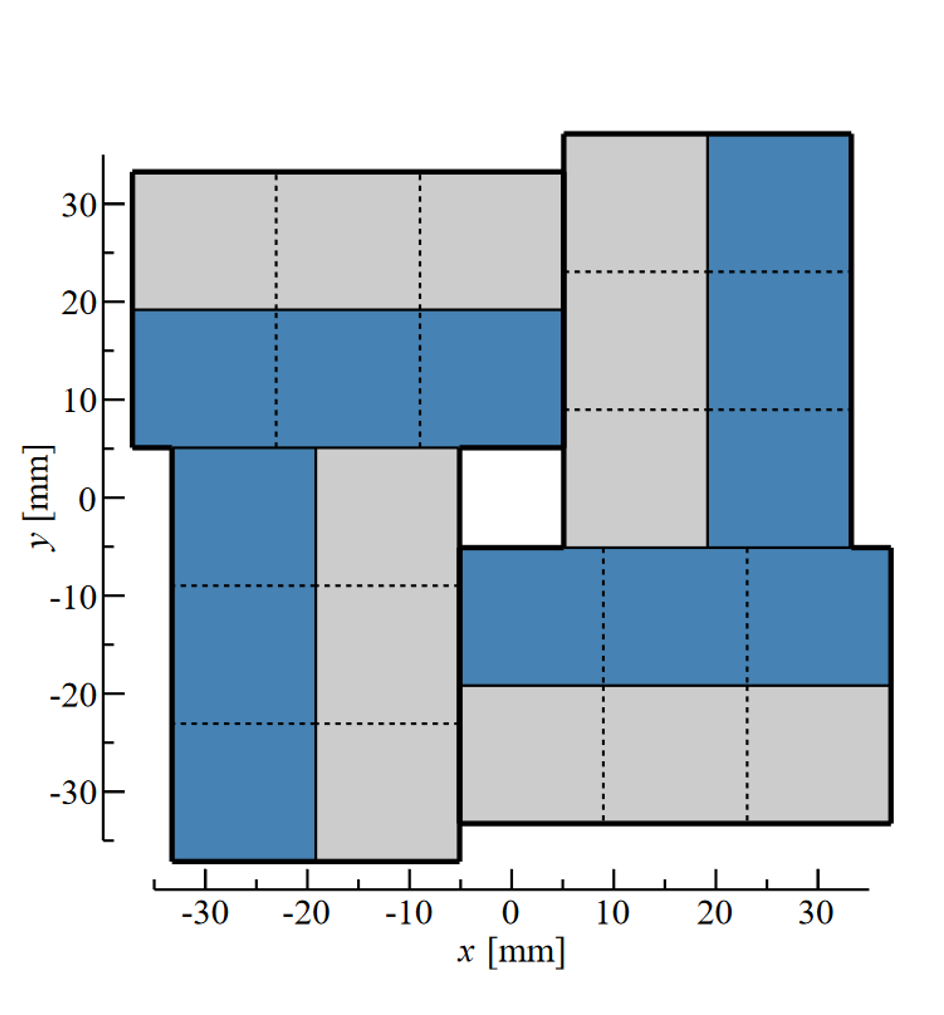
\includegraphics[width=\textwidth]{VeloSensorDiagram}
\caption{Diagram of VELO sensors on each module. Blue sensors are on one side, grey on the other side of the module.} 
\label{fig:VeloSensorDiagram}
\end{subfigure}
\end{figure}


